\documentclass[10pt,norsk,a4paper]{article}
\usepackage[utf8]{inputenc}
\usepackage[T1]{fontenc}
\usepackage[norsk]{babel}
\usepackage[cm]{fullpage}
\usepackage{color}
\usepackage{parskip,textcomp,amssymb,graphicx}
\usepackage{pdfpages}
\usepackage[stable]{footmisc}
\usepackage{multicol}


\title{Generalforsamling \\
	Høst 2019\\[3cm]
	\includegraphics[width=3cm,trim=0 4cm 0 0]{../../res/logo.png}\\}
\date{04.\ November 2019}
\author{Ifi-dagen}

% Blank header, samt footer med side x av y
\usepackage{fancyhdr}
\pagestyle{fancy}
\renewcommand{\headrulewidth}{0pt}
\fancyhead{}
\cfoot{Side~\thepage\ av~\pageref{lastpage}}


\begin{document}

\maketitle{}
\newpage
\part{Dagsorden og detaljer}
\tableofcontents{}
\newpage


\section{Valg av møteleder}

\section{Valg av referent}

\section{Valg av protokollunderskrivere}

\section{Valg av tellekorps}

\section{Godkjenning av innkalling}

\section{Godkjenning av dagsorden}

\section{Årsberetning v/ leder}
Hei Ifi-studenter og foreningsaktive!

\begin{multicols}{2}

Hei ifi-studenter!
Dette året har brakt med seg et par utfordringer og mange gode erfaringer.
Til tross for at styret ikke var fylt før i Februar har vi arrangert ettermidagen@ifi, masterkick-off og dagen@ifi, og tatt med interne på danskebåttur med cybernetisk selskab. 

Høstsemesteret startet med et dynk! Eller flere når vi satt opp dunktank i fadderuka, noe vi håper vil bli en tradisjon fremover. Videre hadde vi også masterkick-off der vi fikk luftet stemningen for alkoholfrie bonger, mottagelsen var blandet, men pizzaen forsvant fort.

Med så mange bedrifter under dagen@ifi ble det også nødvendig å dele opp overansvaret for standene ved å ha bedriftsinterne som bedriftsansvarlige under arrangementet. Vi hadde også flere betalte vektere under kvelden@ifi for å lette på stresset rundt funksjonærkabalen for funksjonæransvarlig.

I år klarte vi og å øke kapasiteten på dagen@ifi fra 54 til hele 64 bedrifter.
Vi hadde også en uvanlig hovedsponsor, nemlig Politiets IKT-tjeneste. De fleste sponosorer er private konsulentfirma, men i år har vi satset på en statlig hovedsponor, og selv om det har medbragt seg litt mer regler har vi satt stor pris på at de satset på oss og har gjennom året også hatt et godt samarbeid.

Dette styret har brukt mer penger for å lette på ansvaret for de forskjellige vervene, til dagen@ifi hadde vi leid inn sceneriggere, lydmann og ekstra vektere, denne kostnaden kommer i tillegg til litt mer penger brukt på interne og litt dyrere funkpakker, men dette er kostnader vi ser på som nyttige for videre utvikling av foreningen.

Det har vært et lærerikt år for alle, spesielt for meg selv som for ca. et år siden påsto at jeg aldri skulle bli leder for noe, men det har vært en ære og et privilegium å bære denne staffettpinnen i 2019.


\end{multicols}

Takk.

Mvh. \\
Kari Eldfrid Stamnes \\
Avtroppende leder \\

\section{Regnskap og revidert budsjett}
Økonomiansvarlig orienterer.

\subsection{Regnskap for 2019}
Økonomiansvarlig legger fram regnskapsresultatet for 2019.

\subsection{Budsjett for 2020}
Økonomiansvarlig legger fram tentativt forslag til budsjett for 2020.

\section{Valg}

\subsection{Leder}
\subsection{Nestleder}
\subsection{Økonomiansvarlig}
\subsection{Bedriftsansvarlig}
\subsection{Faglig ansvarlig}
\subsection{Funksjonæransvarlig}
\subsection{Promoteringsansvarlig}
\subsection{Teknisk ansvarlig}
\subsection{Underholdningsansvarlig}
\subsection{Sosialansvarlig}\label{lastpage}

\newpage
\part{Nåværende vedtekter}
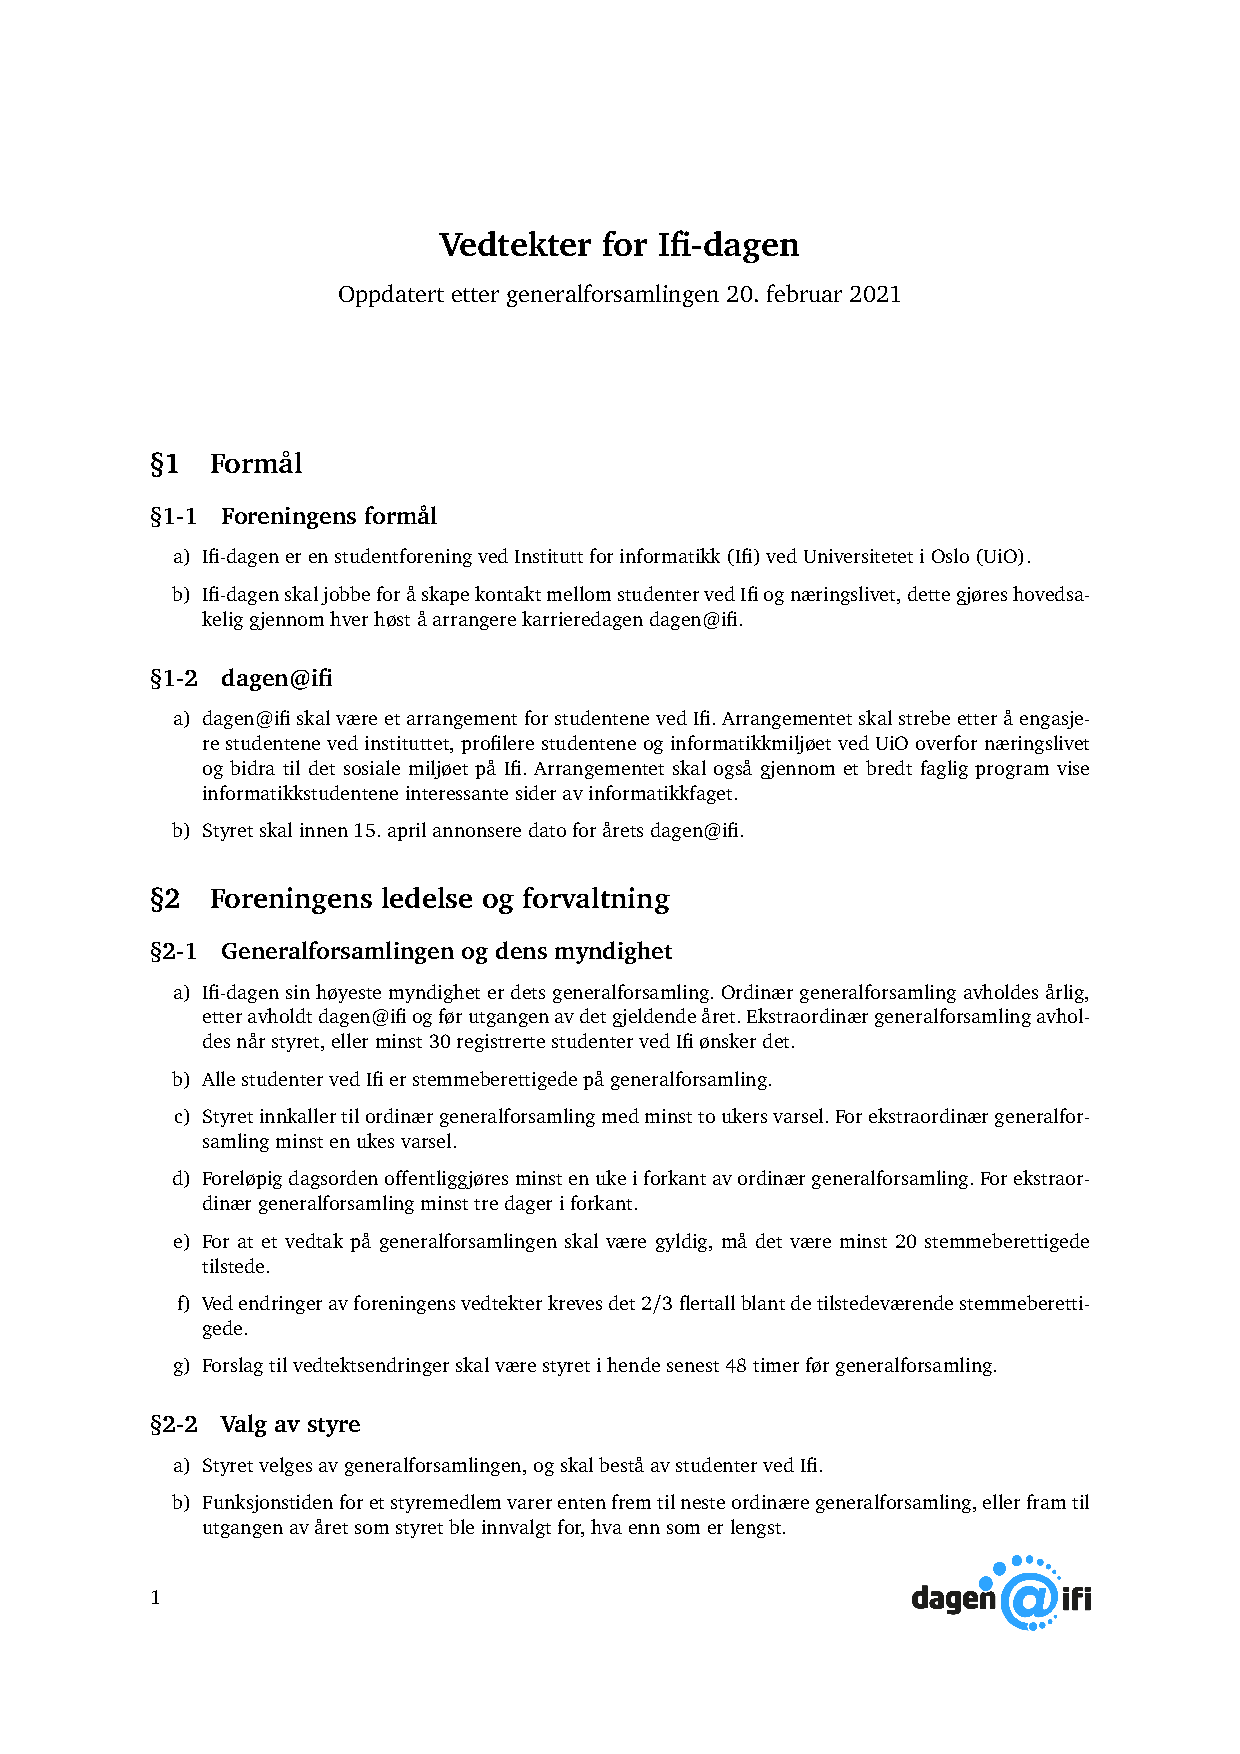
\includepdf[pages=-]{../../vedtekter/vedtekter.pdf}
\end{document}
